\documentclass[12pt]{article}

\usepackage[utf8]{vietnam}
\usepackage[a4paper, top=2.5cm, bottom=2cm, left=3cm, right=3cm]{geometry}
\usepackage{amsmath,amssymb,graphicx}
\usepackage{textalpha}
\usepackage{siunitx}
\usepackage{caption}
\usepackage{subfig}
\usepackage{floatrow}
\usepackage{setspace}
\usepackage{fancyhdr}
\usepackage{indentfirst}

\pagestyle{fancy}
\fancyhf{}
\rhead{Nguyễn Minh Đăng-20230022}
\fancyfoot[C]{\thepage}
\onehalfspacing
\pagenumbering{arabic}


\newfloatcommand{capbtabbox}{table}[][\FBwidth]

\begin{document}

\begin{titlepage}

\newcommand{\HRule}{\rule{\linewidth}{0.5mm}} % Defines a new command for the horizontal lines, change thickness here

\center % Center everything on the page
 
%----------------------------------------------------------------------------------------
%	HEADING SECTIONS
%----------------------------------------------------------------------------------------

\textsc{\LARGE Trường Đại học Khoa học Tự nhiên \\ Đại học Quốc gia TP.HCM}\\[1.5cm] % Name of your university/college

\vspace{3cm}


\textsc{\Large Thực Tập Cơ Sở Kỹ Thuật Hạt Nhân}\\[0.5cm] % Major heading such as course name
%\textsc{\large Assignment 1}\\[0.5cm] % Minor heading such as course title

%----------------------------------------------------------------------------------------
%	TITLE SECTION
%----------------------------------------------------------------------------------------

\HRule \\[0.4cm]
{ \Large \bfseries Bài 1: Các hệ điện tử quan trọng \\ trong thiết bị ghi đo bức xạ hạt nhân}\\[0.4cm] % Title of your document
\HRule \\[1.5cm]
 
%----------------------------------------------------------------------------------------
%	AUTHOR SECTION
%----------------------------------------------------------------------------------------

\begin{minipage}{0.4\textwidth}
\begin{flushleft} \large
\emph{Author: \\ Nguyễn Minh Đăng \\ MSSV: 20230022}\\

\end{flushleft}
\end{minipage}
~
\begin{minipage}{0.4\textwidth}
\begin{flushright} \large
\emph{Lecturer: TS. Võ Hồng Hải} \\
\end{flushright}
\end{minipage}\\[2cm]

% If you don't want a supervisor, uncomment the two lines below and remove the section above
%\Large \emph{Author:}\\
%John \textsc{Smith}\\[3cm] % Your name

%----------------------------------------------------------------------------------------
%	DATE SECTION
%----------------------------------------------------------------------------------------
\vspace{3cm}

{\large \today}\\[2cm] % Date, change the \today to a set date if you want to be precise

%----------------------------------------------------------------------------------------
%	LOGO SECTION
%----------------------------------------------------------------------------------------

 % Include a department/university logo - this will require the graphicx package
 
%----------------------------------------------------------------------------------------

\vfill % Fill the rest of the page with whitespace

\end{titlepage}

\section{Lý Thuyết}

\subsection{Trình bày nguyên lý hoạt động hệ đo phổ gamma}

\indent Khi các bức xạ gamma tương tác với đầu dò NaI(Tl) sẽ tạo ra các xung điện với biên độ nhỏ. Các xung điện này được đưa qua bộ tiền khuếch đại và khuếch đại để điều chỉnh là phóng đại xung. Sau đó, chúng sẽ được đưa vào bộ phân tích xung hoặc bô phân tích đa kênh MCA. Sau khi MCA nhận được các tín hiệu xung từ đầu dò chúng sẽ qua bộ ADC (Analogy Digiltal Converter) đây là bộ chuyển đổi tín hiệu analogy thành tín hiệu digiltal. Sau khi có được các tín hiệu số thì MCA sẽ lưu trữ và xử lí và thể hiện ra màn hình máy tính để người thực hiện có thể quan sát một cách dễ dàng.

\subsection{Trình bày nguyên lý hoạt động của hệ đo số đếm}

\indent Khi các hạt tích điện dịch chuyển trong chất khí, nó sẽ ion hoá các phân tử chất khí dọc theo đường đi của nó - tạo ra các ion mang điện dương và các electron tự do được gọi là cặp ion - electron. Các ion có thể được tạo ra do tương tác giữa phân tử với hạt mang điện hoặc do va chạm với các hạt mang điện thứ cấp được tạo ra từ quá trình ion hoá sơ cấp. Ở đây ta không quan tâm đến năng lượng cơ học của electron hay ion nhận được do va chạm mà chủ yếu chỉ quan tâm đến số cặp ion được tạo ra dọc theo đường đi của hạt bức xạ.  Một Detector chứa khí đơn giản chỉ gồm một ống chứa khí và hai điện cực, thành của ống chứa khí được thiết kế để cho bức xạ cần ghi có thể đi được vào phía bên trong.

\subsection{Hãy trình bày chức năng của Oscilloscope trong điện tử hạt nhân}

\indent Kiểm tra, điều chỉnh và hiển thị tín hiệu điện áp dưới dạng sóng, biểu diễn trực quan về sự thay đổi của điện áp theo thời gian. Các tín hiệu được vẽ trên biểu đồ, cho biết tín hiệu thay đổi như thế nào. Từ việc quan sát được các tín hiệu điện trên máy hiện sóng sẽ giúp chúng ta có thể phân tích, đánh giá được tình trạng của thiết bị, tình trạng hoạt động, mức độ nhiễu sóng… và có hướng điều chỉnh sao cho hợp lý .

\newpage
\subsection{Hãy phối hợp trở kháng giữa thiết bị (1) có trở kháng $\mathbf{Z}_\mathbf{1}=\mathbf{50}\mathbf{\Omega}$ kết nối với thiết bị (2) có trở kháng $\mathbf{Z}_\mathbf{2}=\mathbf{1}\mathbf{M\Omega}$}

\begin{figure}[h]
	\includegraphics[width=\textwidth]{mach dien}
\end{figure}

\newpage \section{Kết Quả Thực Nghiệm}

\subsection{Trình bày kết quả phổ năng lượng của các nguồn chuẩn đã đo (phổ số đếm theo kênh).}
\subsubsection{Nguồn: Eu-152, đồng vị phóng xạ của europium Eu-63}

\begin{figure}[h]
	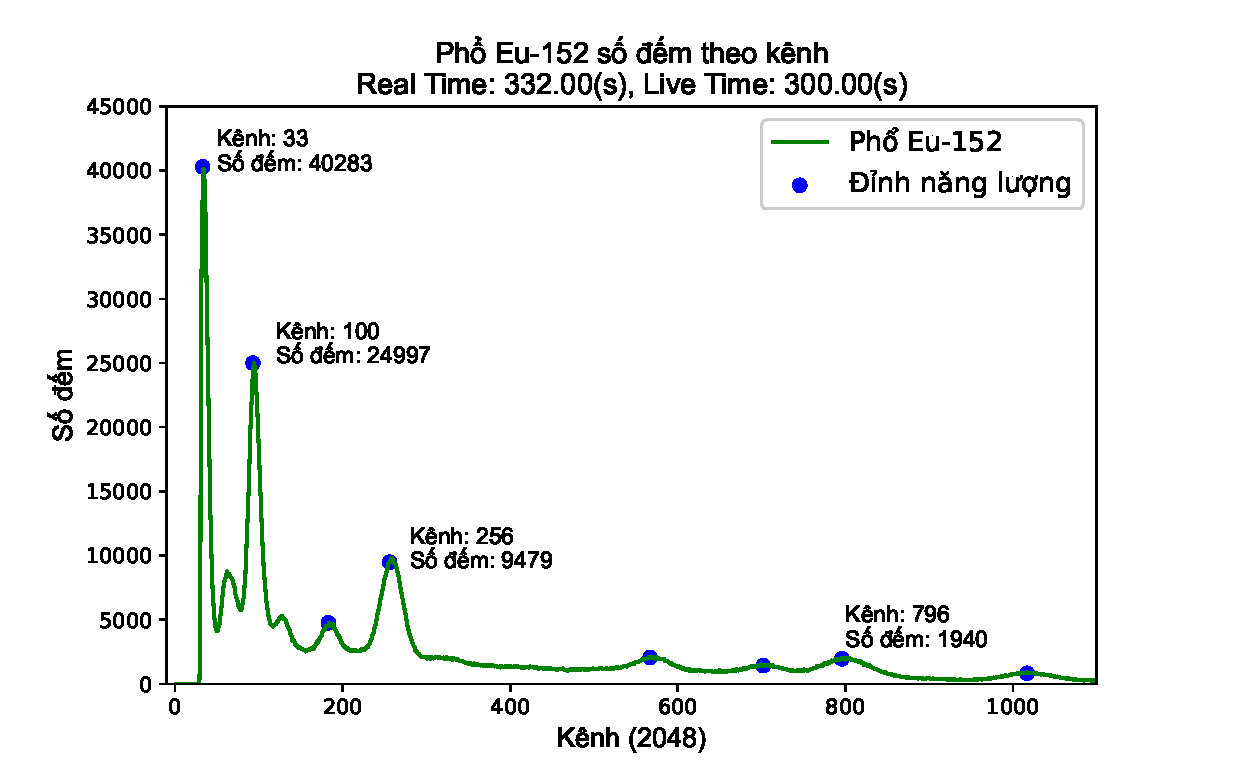
\includegraphics[width=\textwidth]{Eu-152-Plot_cn}
	\caption{Đồ thị số đếm theo kênh Eu-152}
\end{figure}

\newpage
\subsubsection{Nguồn: Ba-133 đồng vị phóng xạ của barium Ba-56}

\begin{figure}[!th]
	\includegraphics[width=\textwidth]{Ba-133-Plot_cn}
	\caption{Đồ thị số đếm theo kênh Ba-133}
\end{figure}

\subsubsection{Nguồn: Co-60, Cobalt-60}

\begin{figure}[!th]
	\includegraphics[width=\textwidth]{Co-60-Plot_cn}
	\caption{Đồ thị số đếm theo kênh Co-60}
\end{figure}

\newpage
\subsection{ Trình bày kết quả chuẩn năng lượng theo kênh (trình bày đường chuẩn năng lượng và phương trình chuẩn năng lượng). Ở đó, phương trình chuẩn năng lượng có dạng $\mathbf{E(keV) = a.channel + b}$}

Từ các số liệu trên ta có các đỉnh

\begin{table}[!ht]
    \centering
    \begin{tabular}{cccccc}
    \hline
        \textbf{Eu-152} & \textbf{} & \textbf{Ba-133} & \textbf{} & \textbf{Co-60} & \textbf{} \\ \hline
        Năng lượng (keV) & Kênh & Năng lượng (keV) & Kênh & Năng lượng (keV) & Kênh \\ 
        121.7817 & 93 & 80.9979 & 66 & 1173.228 & 851 \\ 
        244.6974 & 183 & 302.8508 & 242 & 1332.492 & 962 \\ 
        344.2785 & 256 & 356.0129 & 287 & ~ & ~ \\ 
        778.9045 & 567 & ~ & ~ & ~ & ~ \\ 
        964.079 & 702 & ~ & ~ & ~ & ~ \\ 
        1112.076 & 796 & ~ & ~ & ~ & ~ \\ 
        1408.013 & 1017 & ~ & ~ & ~ & ~ \\ 
        ~ & ~ & ~ & ~ & ~ & ~ \\ \hline
    \end{tabular}
\end{table}

\begin{figure}[h!]
	\includegraphics[width=\textwidth]{Peak-Plot_cn}
	\caption{Đồ thị phương trình chuẩn năng lượng}
\end{figure}

\newpage
\subsection{Trình bày kết quả phổ năng lượng sau khi đã chuẩn năng lượng (phổ số đếm theo năng lượng)}

Từ phương trình tuyến tính: $E = 1.41$$\times$kênh$-20.66$ $(keV)$ \\

\indent Ta có thể suy ra các phổ năng lượng \\

Ta có dữ liệu từ LaraWeb

\begin{table}[!ht]
    \centering
    \resizebox{\columnwidth}{!}{
    \begin{tabular}{ccccccc}
    \hline
         Energy (keV)  &  Intensity (\%)  &  Type  &  Origin* &   Levels   & ~ &   Possible coincidence with (keV) /  \\ \hline
        ~ & ~ & ~ & ~ &  Start* &   End*  &  Possible sum of (levels)   \\ 
            40.1186 (-) &     37.7 (5) &  XKα1  &  Sm  &    &    & ~ \\ 
           121.7817 (3) &     28.41 (13) &  γ   &  Sm-152  &  1  &  0  & ~ \\ 
           344.2785 (12) &     26.59 (12) &  γ   &  Gd-152  &  1  &  0  & ~ \\ 
         1 408.013 (3) &     20.85 (8) &  γ   &  Sm-152  &  13  &  1  & ~ \\ 
           964.079 (18) &     14.50 (6) &  γ   &  Sm-152  &  9  &  1  & ~ \\ 
         1 112.076 (3) &     13.41 (6) &  γ   &  Sm-152  &  10  &  1  & ~ \\ 
           778.9045 (24) &     12.97 (6) &  γ   &  Gd-152  &  7  &  1  & ~ \\ 
           244.6974 (8) &      7.55 (4) &  γ   &  Sm-152  &  2  &  1  & ~ \\ \hline
    \end{tabular}
    }
\end{table}

\begin{figure}[!h]
	\includegraphics[width=\textwidth]{Peak-Eu-152-Plot_cn}
	\caption{Đồ thị số đếm theo năng lượng Eu-152}
\end{figure}

\newpage

Ta có dữ liệu từ LaraWeb

\begin{table}[!ht]
    \centering
    \resizebox{\columnwidth}{!}{
    \begin{tabular}{ccccccc}
    \hline
         Energy (keV)  &  Intensity (\%)  &  Type  &  Origin* &   Levels   & ~ &   Possible coincidence with (keV) /  \\ \hline
        ~ & ~ & ~ & ~ &  Start* &   End*  &  Possible sum of (levels)   \\ 
            30.9731 (-) &     62.4 (7) &  XKα1  &  Cs  &    &    & ~ \\ 
           356.0129 (7) &     62.05 (19) &  γ   &  Cs-133  &  4  &  1  &  80.9980 (Σ=437.0100) \\ 
            30.6254 (-) &     33.8 (4) &  XKα2  &  Cs  &    &    & ~ \\ 
            80.9979 (11) &     33.31 (30) &  γ   &  Cs-133  &  1  &  0  &  356.0130 (Σ=437.0100) \\ 
           302.8508 (5) &     18.31 (11) &  γ   &  Cs-133  &  3  &  1  & ~ \\ 
            35.053 (-) &     18.24 (29) &  XK'β1  &  Cs  &    &    & ~ \\ 
             4.67355 (-) &     15.87 (26) &  XL  &  Cs  &    &    & ~ \\ 
           383.8485 (12) &      8.94 (6) &  γ   &  Cs-133  &  3  &  0  & ~ \\ 
           276.3989 (12) &      7.13 (6) &  γ   &  Cs-133  &  4  &  2  & ~ \\ 
            35.9003 (-) &      4.45 (12) &  XK'β2  &  Cs  &    &    & ~ \\ 
            79.6142 (19) &      2.63 (19) &  γ   &  Cs-133  &  2  &  1  & ~ \\ 
            53.1622 (18) &      2.14 (6) &  γ   &  Cs-133  &  4  &  3  & ~ \\ 
           160.6121 (16) &      0.638 (6) &  γ   &  Cs-133  &  2  &  0  & ~ \\ 
           223.2368 (13) &      0.450 (5) &  γ   &  Cs-133  &  3  &  2  & ~ \\ \hline
    \end{tabular}
    }
\end{table}

\begin{figure}[!h]
	\includegraphics[width=\textwidth]{Peak-Ba-133-Plot_cn}
	\caption{Đồ thị số đếm theo năng lượng Ba-133}
\end{figure}

\newpage

Ta có dữ liệu từ LaraWeb

\begin{table}[!th]
    \centering
    \resizebox{\columnwidth}{!}{
    \begin{tabular}{ccccccc}
    \hline
        Energy (keV)  &  Intensity (\%)  &  Type  &  Origin* &   Levels   & ~ &   Possible coincidence with (keV) /  \\ \hline
        ~ & ~ & ~ & ~ &  Start* &   End*  &  Possible sum of (levels)   \\ 
         1 332.492 (4) &     99.9826 (6) &  γ   &  Ni-60  &  1  &  0  &  1 173.228 (Σ=2 505.720) \\ 
         1 173.228 (3) &     99.85 (3) &  γ   &  Ni-60  &  3  &  1  &  1 332.492 (Σ=2 505.720) \\ 
           826.10 (3) &      0.0076 (8) &  γ   &  Ni-60  &  2  &  1  & ~ \\ 
           347.14 (7) &      0.0075 (4) &  γ   &  Ni-60  &  3  &  2  & ~ \\ 
             7.47824 (-) &      0.0065 (3) &  XKα1  &  Ni  &    &    & ~ \\ 
             7.46097 (-) &      0.00334 (12) &  XKα2  &  Ni  &    &    & ~ \\ 
             8.2967 (-) &      0.00136 (5) &  XK'β1  &  Ni  &    &    & ~ \\ 
         2 158.57 (3) &      0.0012 (2) &  γ   &  Ni-60  &  2  &  0  & ~ \\ 
             0.84 (-) &      0.0002 (-) &  XL  &  Ni  &    &    & ~ \\ 
         2 505.692 (5) &      0.0000020 (4) &  γ   &  Ni-60  &  3  &  0  &  (3→1)+(1→0) \\ \hline
    \end{tabular}
    }
\end{table}
\begin{figure}[!ht]
	\includegraphics[width=\textwidth]{Peak-Co-60-Plot_cn}
	\caption{Đồ thị số đếm theo năng lượng Co-60}
\end{figure}

\newpage
\subsection{Trình bày kết quả đo phổ năng lượng phông môi trường.}

Ta có số phổ phông môi trường như sau

\begin{figure}[h!]
	\includegraphics[width=\textwidth]{Peak-bg}
	\caption{Phổ năng lượng môi trường}
\end{figure}


\end{document}
